% Arara is a cross-platform automation tool to build pdf what follows are the build rules 
% arara: pdflatex: { synctex: on }
% arara: biber
% arara: makeglossaries
% arara: makeindex
% arara: pdflatex: { synctex: on }
% arara: pdflatex: { synctex: on }

\documentclass[titlepage,11pt]{article}
\usepackage[utf8]{inputenc}     %UTF8 encoding
\usepackage[margin=1in]{geometry}     %margins 


\usepackage{tocbibind}  % Genereate TOC which includes figures,bib,etc
\usepackage{times}  %use times font, looks better 
\usepackage{setspace} %set double space and single space
\usepackage{float}   % Better floating and positioning
\usepackage{wrapfig}   % Wrap text around figures
\usepackage{graphicx}   %include images
\usepackage{subcaption} % subcaption images
\usepackage[pdftex,hidelinks]{hyperref} % use href links, good practise to import it last

%bibleography
\usepackage[backend=biber,backref]{biblatex}
\addbibresource{references.bib}

\usepackage{imakeidx} % Genereate index of terms
\makeindex[columns=3, columnseprule, title=Alphabetical Index, intoc]


\usepackage{booktabs} % For \toprule, \midrule and \bottomrule
\usepackage{siunitx} % Formats the units and values
\usepackage{pgfplotstable} % Generates table from .csv
\pgfplotsset{compat=1.16}
% Setup siunitx:
\sisetup{
	round-mode          = places, % Rounds numbers
	round-precision     = 2, % to 2 places
}

\usepackage{blindtext}
\usepackage{listings} % style source code
\usepackage{color}
\definecolor{dkgreen}{rgb}{0,0.6,0}
\definecolor{gray}{rgb}{0.5,0.5,0.5}
\definecolor{mauve}{rgb}{0.58,0,0.82}



\lstset{frame=tb,
	aboveskip=3mm,
	belowskip=3mm,
	showstringspaces=false,
	columns=flexible,
	basicstyle={\small\ttfamily},
	numbers=left,
	numberstyle=\tiny\color{gray},
	keywordstyle=\color{blue},
	commentstyle=\color{dkgreen},
	stringstyle=\color{mauve},
	breaklines=true,
	breakatwhitespace=true,
	tabsize=4
}

% glossaries
\usepackage[toc]{glossaries}
\setglossarystyle{listgroup} 
\setacronymstyle{long-short}
\makeglossaries
\loadglsentries{glossary} % load glossaries from glossary.tex file




\title{
	Machine Learning Mini Project 1 \\
	Humidity Prediction Based on Weather History \thanks{Instructor: Anthony Sander}
}

\author{Faisal Ahmed \and Mustafizur Rahman Hilaly}
\date{\today}


\begin{document}
\maketitle
\tableofcontents


\begin{abstract}
\addcontentsline{toc}{section}{Abstract}
In this project, we are predicting humidity based on historical weather data. To do so, we initially performed Exploratory Data Analysis (EDA) on the dataset to select appropriate features for the machine learning models. We evaluated our dataset on five different classifiers and observed prediction scores from the classifiers. We also plotted Learning curves and Validation curves of 5 different classifiers. To cross-check our findings, we fitted our data to AutoML to get the best estimator from AutoML.
	 
From this experiment, we came up with the best performing estimator for our dataset and then used Grid Search to tune its hyperparameters to get the most optimum result from the model. We then plotted the ROC-AUC curve to visualize the performance of different estimators. Finally, we applied Principal Component Analysis PCA to analyze dimensionality reduction.\end{abstract}

\section{Exploratory Data Analysis (EDA) \& Data Preparation}
Initially, we checked the shape, information, and statistics of the dataset to have a better understanding of the data.  That helped us to figure out the features and target variables.  Before proceeding further we had to clean up the data for use. To do so, we first identified and removed all the unnecessary columns from the dataset, then we checked null values and fill them with approximate values.  In our data set, there was a categorical value (“Precip Type”) which we encoded to numeric value using one-hot encoding technique. 

After the initial processing, we plotted box and scatter plots to have more understanding of the data. We then split the whole dataset into 80:20 split for training and testing respectively.

\begin{figure}[h]
\centering
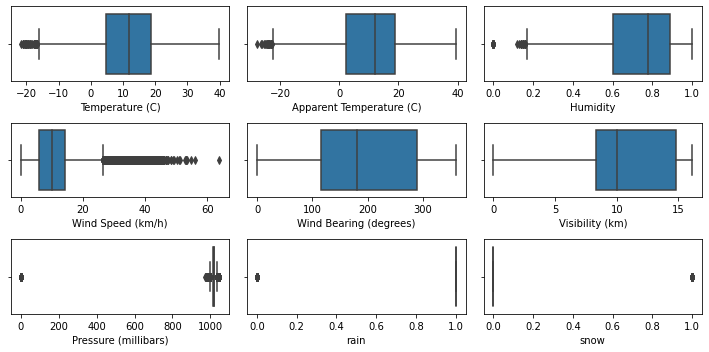
\includegraphics[width=.92\linewidth]{boxplot}
\caption{Box Plot}%
\label{fig:boxplot}
\end{figure}

\begin{figure}[h]
\centering
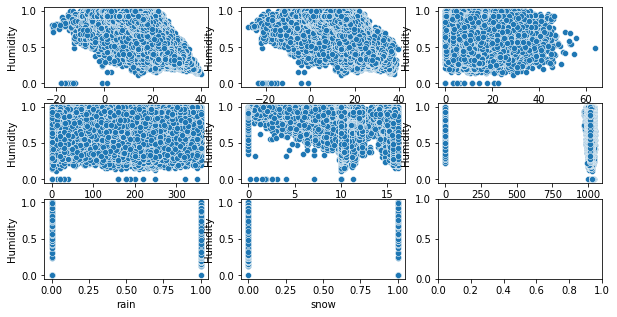
\includegraphics[width=.92\linewidth]{scatterplot}
\caption{Scatter Plot}%
\label{fig:scatterplot}
\end{figure}


\section{Experiment with Different Classification Models}
To perform our experiment, we selected five different classification modes.
\begin{enumerate}
\item Logistic Regression
\item Decision Tree Classifier
\item K Nearest Neighbor
\item Gradient Boosting (we didn’t study this one in the class)
\item Random Forest
\end{enumerate}
For every model, we fitted training data and measured their performance against test data. We also plotted validation and learning curves for each model to understand their behavior better.

As every model is biased, we fitted all of the previously mentioned models inside the Voting Classifier to get a more realistic result.

To get the best out of the individual model, we selected the best-performing model from the list of five models and applied Grid Search to tune its hyperparameters.

Finally, we fitted our dataset into AutoML to get the best model for our selected dataset. We used TPOT as the AutoML library.

\subsection{Logistic Regression}
We observed 80.05% accuracy using Logistic Regression
\begin{figure}[h]
\centering
\begin{subfigure}[b]{0.45\linewidth}
    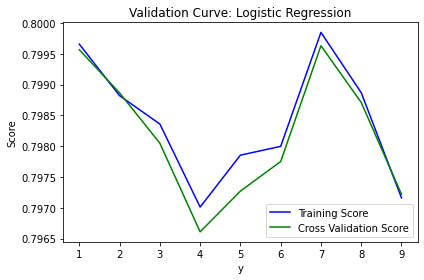
\includegraphics[width=\linewidth]{lrvc}
    \caption{Logistic Regression Validation Curve.}
\end{subfigure}
\begin{subfigure}[b]{0.45\linewidth}
    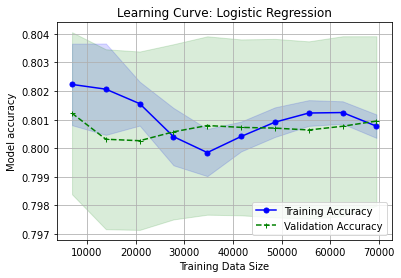
\includegraphics[width=\linewidth]{lrlc}
    \caption{Logistic Regression Learning Curve.}
\end{subfigure}
\end{figure}

\clearpage

\subsection{Decision Tree Classifier}
We observed 81.04% accuracy using Decision Tree Classifier
\begin{figure}[h]
\centering
\begin{subfigure}[b]{0.45\linewidth}
    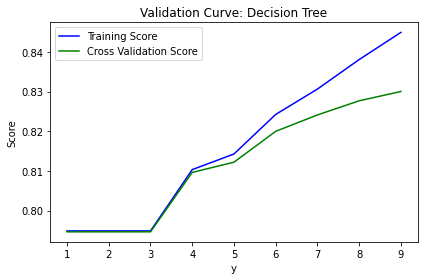
\includegraphics[width=\linewidth]{dtcvc}
    \caption{Decision Tree Classifier Validation Curve.}
\end{subfigure}
\begin{subfigure}[b]{0.45\linewidth}
    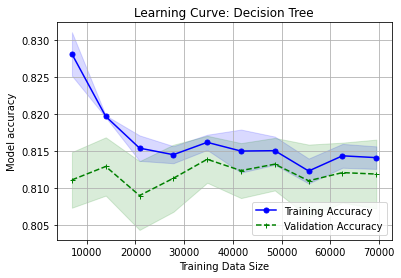
\includegraphics[width=\linewidth]{dtclc}
    \caption{Decision Tree Classifier Learning Curve.}
\end{subfigure}
\end{figure}


\subsection{K Nearest Neighbor}
We observed 82.62 % accuracy using K Nearest Neighbor
\begin{figure}[h]
\centering
\begin{subfigure}[b]{0.45\linewidth}
    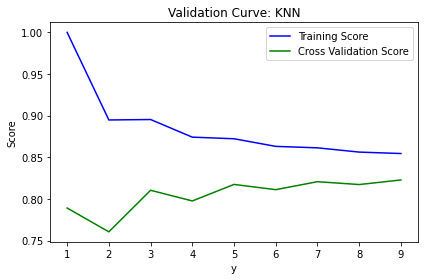
\includegraphics[width=\linewidth]{knnvc}
    \caption{K Nearest Neighbor Validation Curve.}
\end{subfigure}
\begin{subfigure}[b]{0.45\linewidth}
    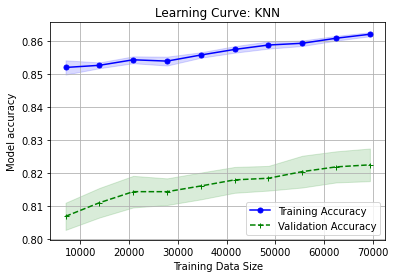
\includegraphics[width=\linewidth]{knnlc}
    \caption{K Nearest Neighbor Learning Curve.}
\end{subfigure}
\end{figure}

\clearpage

\subsection{Random Forest}
We observed 83.94 % accuracy using Random Forest
\begin{figure}[h]
\centering
\begin{subfigure}[b]{0.45\linewidth}
    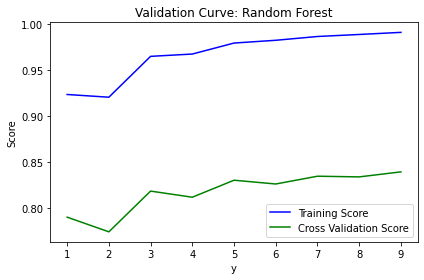
\includegraphics[width=\linewidth]{rfvc}
    \caption{Random Forest Validation Curve.}
\end{subfigure}
\begin{subfigure}[b]{0.45\linewidth}
    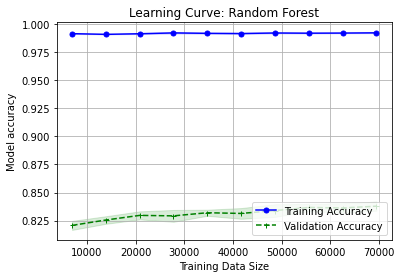
\includegraphics[width=\linewidth]{rflc}
    \caption{Random Forest Learning Curve.}
\end{subfigure}
\end{figure}

\subsection{Gradient Boosting}
Gradient Boosting wast the best performing model of all and we We observed 84.72% accuracy using Logistic Regression.
\begin{figure}[h]
\centering
\begin{subfigure}[b]{0.45\linewidth}
    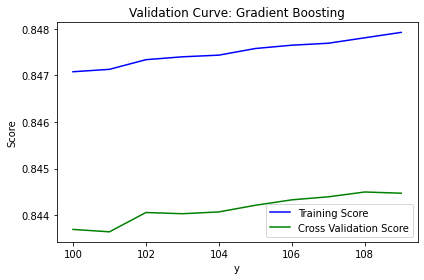
\includegraphics[width=\linewidth]{gbcvc}
    \caption{Gradient Boosting Validation Curve.}
\end{subfigure}
\begin{subfigure}[b]{0.45\linewidth}
    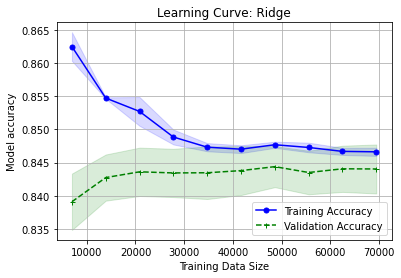
\includegraphics[width=\linewidth]{gbclc}
    \caption{Gradient Boosting Curve.}
\end{subfigure}
\end{figure}

\subsection{Voting Classifier}

When we combined all the models and fitted into voting classifier we observed slightly better result than the individual best performing model (Gradient Boosting). We observed 84.97 %  accuracy, which is .25 % increase in accuracy.

\subsection{AutoML with TPOT}
As it takes very long time to figure out the right model automatically using AutoML, we interrupted the TPOT in the middle of its execution. Even we didn’t let AutoML to finish still we got Random Forest Classifier as the best performing model. Which is pretty close to our final result. Random Forest Classifier was the second best performing model for our data set.

\subsection{Grid Search to Tune Gradient Boosting}
We ran grid search with selective hyper parameters of Gradient Boosting to figure out best possible hyper parameters for our problem

\lstinputlisting[language=Python]{demo-python.py}

\subsection{AUC-ROC Curve}
We plotted AUC-ROC curve to visualize our result
\begin{figure}[h]
\centering
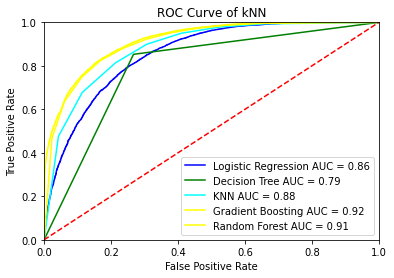
\includegraphics[width=.92\linewidth]{aucroc}
\caption{AUC-ROC Curve}%
\label{fig:aucroc}
\end{figure}

\clearpage

\subsection{Principal Component Analysis(PCA)}
Finally we performed PCA for dimensionality reduction.
\begin{figure}[h]
\centering
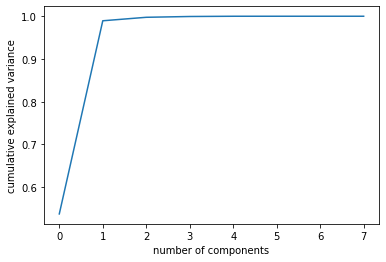
\includegraphics[width=.92\linewidth]{pca}
\caption{PCA}%
\label{fig:pca}
\end{figure}


\section{Conclusion}
From this experiment we found that Gradient Boosting’s performance is very good but it takes long time to train the model. We also found that Voting Classifier works very well to increase overall performance. 
And Finally, AutoML is very powerful but it requires lot of time and resources to generate best performing estimator. 

\end{document}
